\documentclass[12pt]{beamer}
\usetheme[navbar=false, bkgimage=false, shadow=true]{Fermi}

%  \begin{columns}
%    \column{0.5\textwidth}
%    \column{0.5\textwidth}
%  \end{columns}

\usepackage{graphicx}

\usepackage{amsmath}


% taken from http://da.vidr.cc/2008/09/29/creating-flowcharts-with-pgftikz-in-latex/
\usepackage{tikz}
\usetikzlibrary{shapes,arrows}
\tikzstyle{decision} = [diamond, draw, text width=4.5em, text badly centered, node distance=3cm, inner sep=0pt]
\tikzstyle{block} = [rectangle, draw, text width=5em, text centered, rounded corners, minimum height=4em]

\title{A New Maximum Likelihood Method for Defining the pulsar off-peak}
%\subtitle{\ldots}

\author{Joshua Lande}

\institute{
With much help from Damien + Matthew\\[1em]
SLAC/Stanford}
\email{joshualande@gmail.com}
\date{August 25, 2011}

\begin{document}

\fermititle

\begin{frame}{Motivation}
  \begin{itemize}
    \item Most People like to study where the pulsar is
    \item But many reason to want to know where (in phase) the pulsar is not
      \begin{itemize}
        \item Studying nearby sources which may be confused $\rightarrow$ $\gamma$-Cgygni SNR
        \item Off-peak emission (or lack therefo) is interesting for pulsar modeling  $\rightarrow$ CTA1
        \item Looking for DC emission from the pulsar's wind $\rightarrow$ PWNCAT2
      \end{itemize}
  \end{itemize}
\end{frame}

\begin{frame}{What has been done before}

  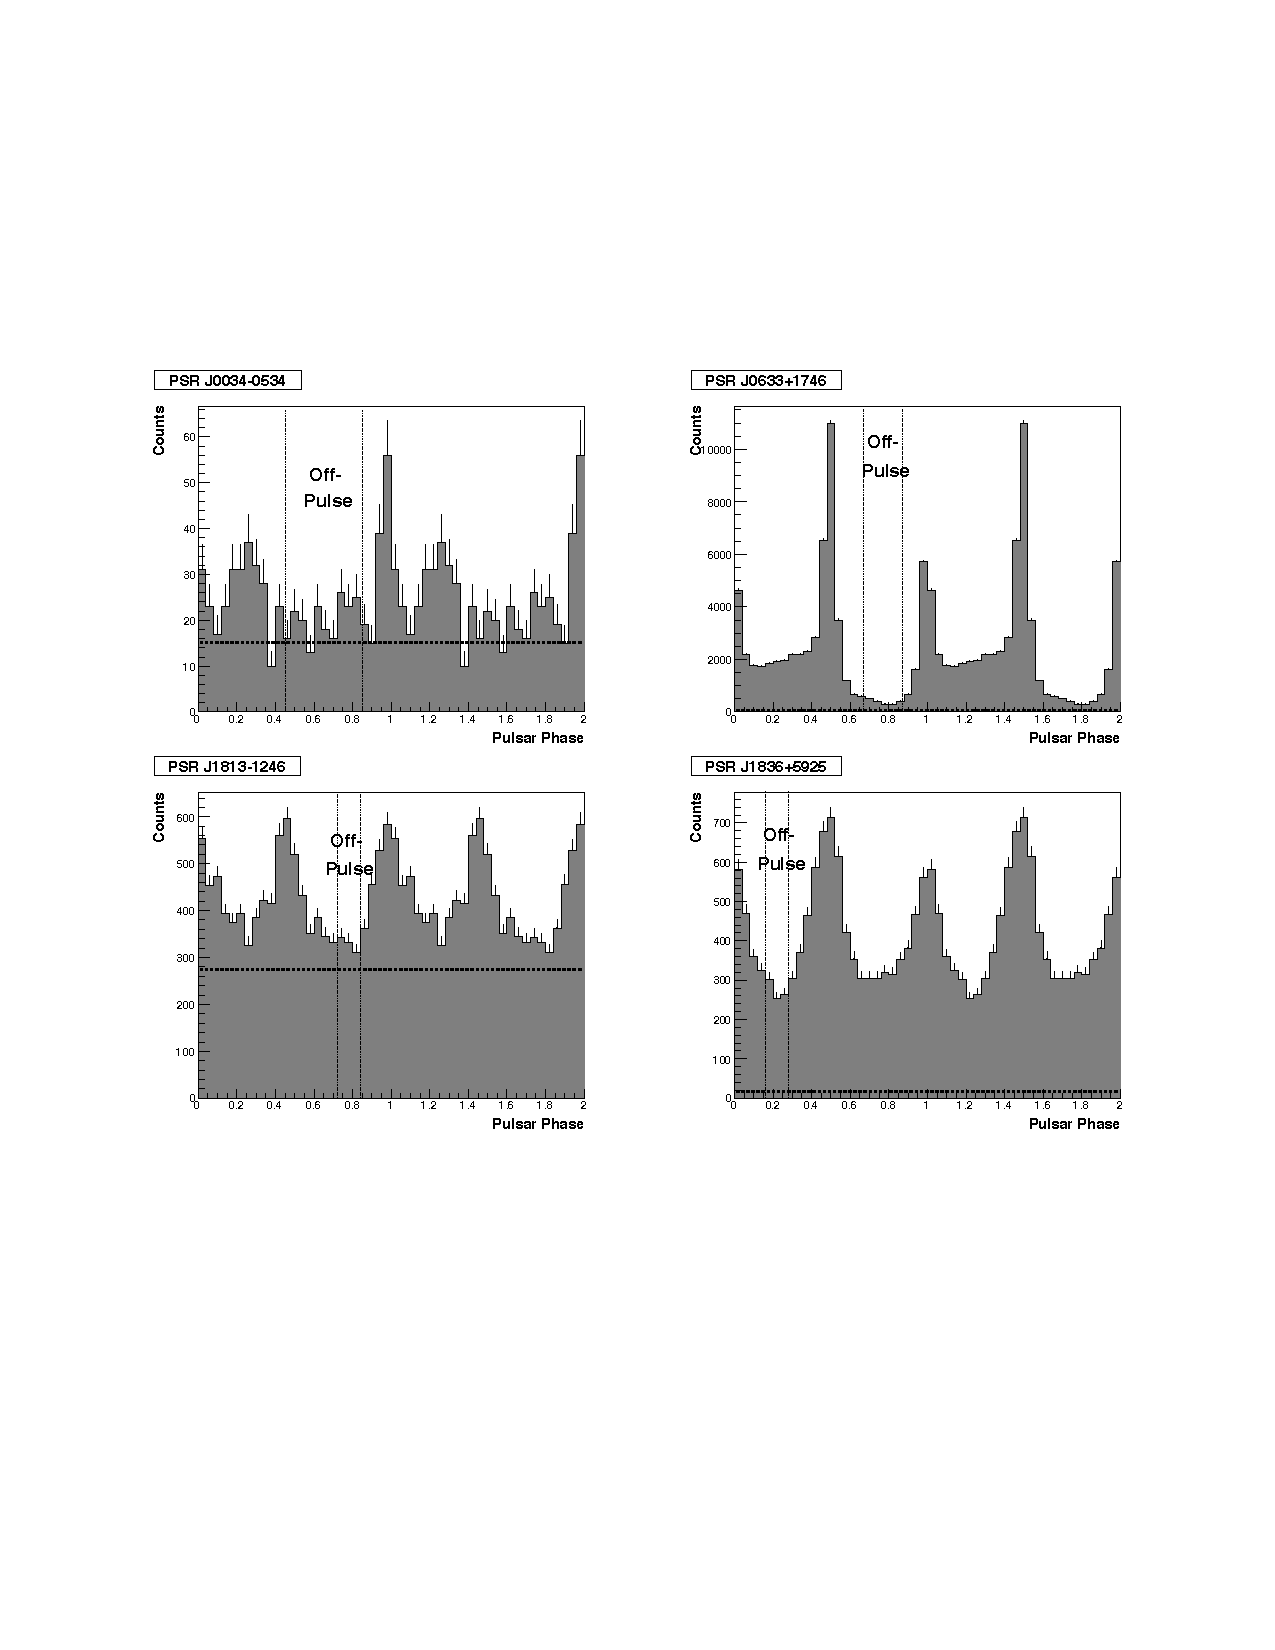
\includegraphics[width=0.75\textwidth]{plots/off_pulse_pwncat1.pdf}

  \begin{itemize}
    \item PWNCat1 $\rightarrow$ Selected by eye from pulsar phaseogram.
    \item Method validated by large scale spectral analysis
  \end{itemize}
\end{frame}

\begin{frame}{Another Method: CTA1-Paper II}

  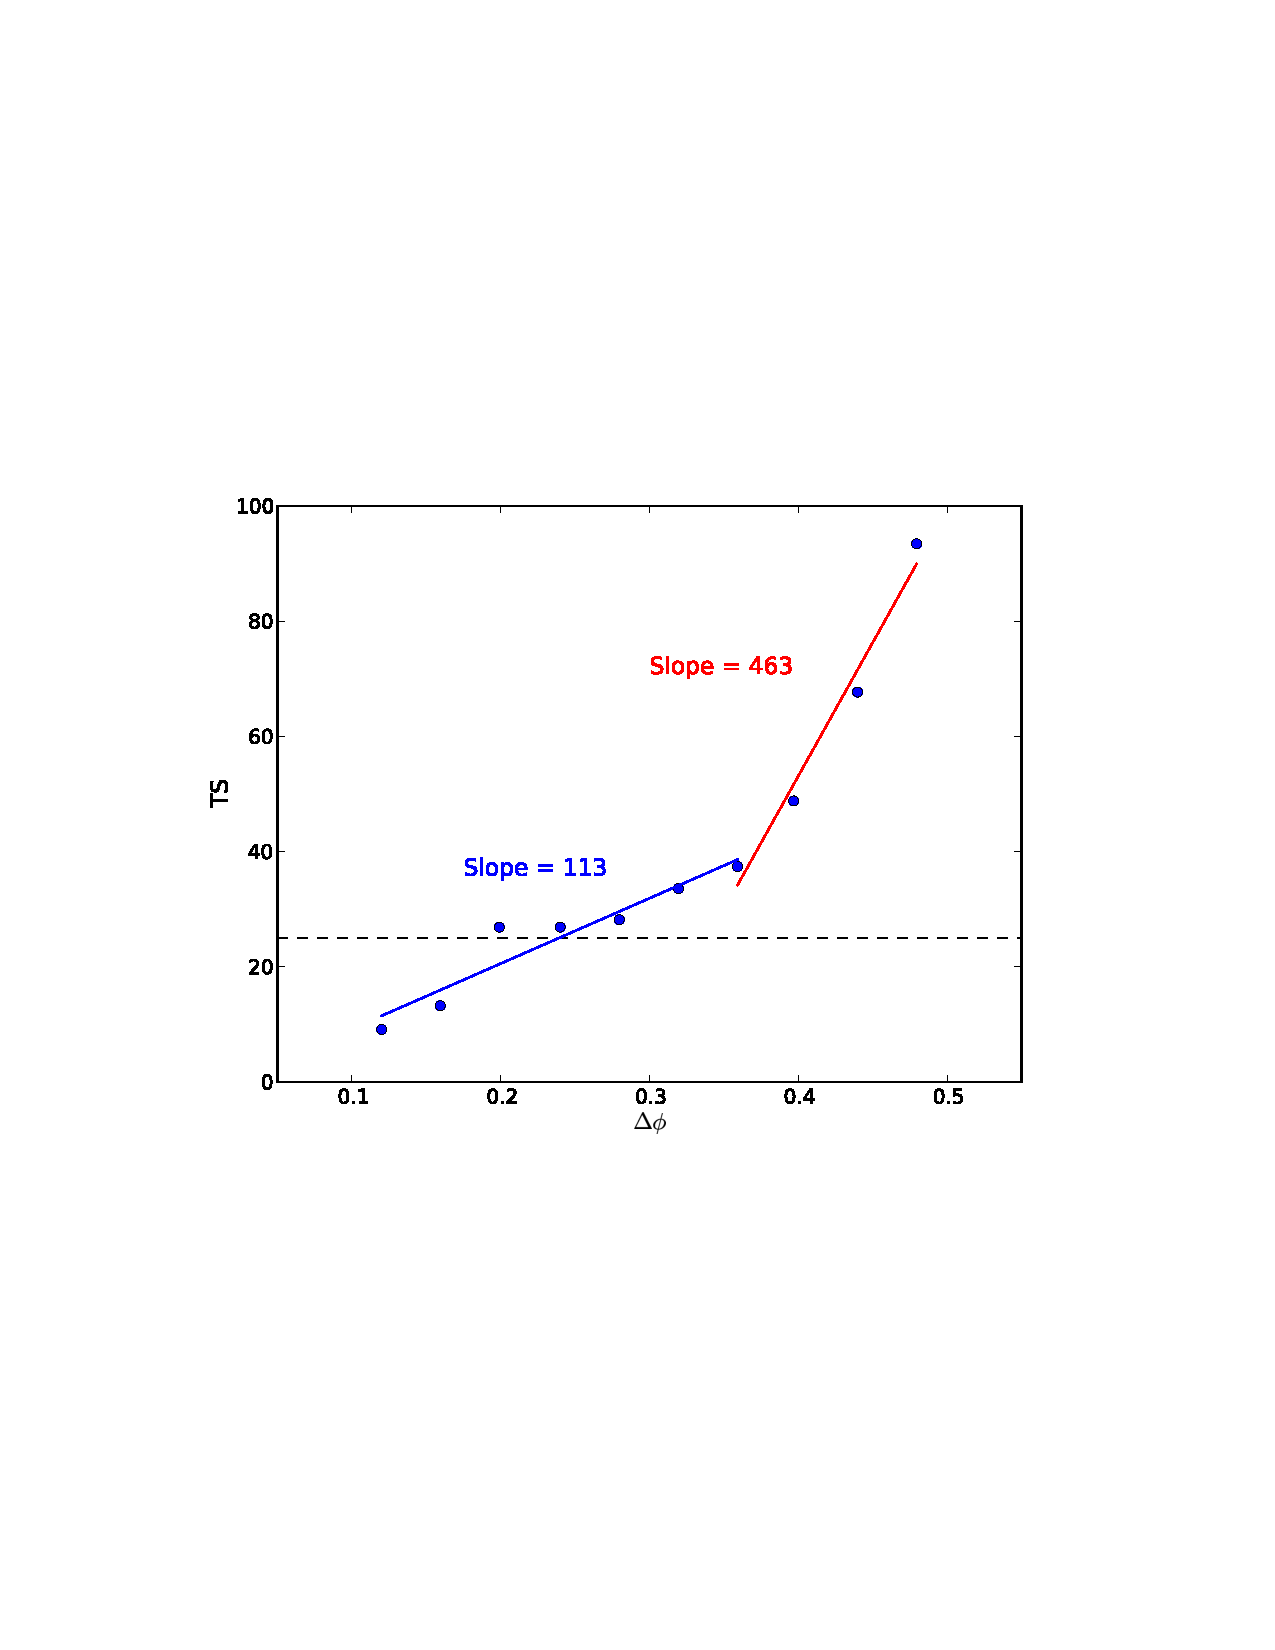
\includegraphics[width=0.75\textwidth]{plots/cta1.pdf}

  2nd CTA1 Paper$\rightarrow$ Look for break in TS vs $\Delta \phi$

\end{frame}

\begin{frame}{Maximum likelihood pulsar fitting}
  \begin{itemize}
    \item Any New Idea's for defining the off-peak?
    \item Matthe gave me a new idea:
      \begin{itemize}
   \item \texttt{uw.pulsar} for maximum likelihood fitting of pulsar light curves
   \item Has to be done anyway for 2nd pulsar catalog (Damien + Matthew)
     do define the peak separations
   \item Can we use the best fit light curve to define the off peak?
  \end{itemize}
  \end{itemize}
\end{frame}

\begin{frame}{\texttt{uw.pulsar}, under the hood}
  \begin{itemize}
   \item Define the unbinned likelihood: $\mathcal{L} = \sum_\text{photons}\text{PDF}(\text{phase})$
   \item Here, $\text{PDF}=\text{PDF}(\text{model parameters})$, so you have to pick a pulsar light curve model!
   \item As usual, maximize the log of the Likelihood
  \end{itemize}

  Example:\footnote{From \url{https://confluence.slac.stanford.edu/x/2AIyAw}}
  \begin{columns}
    \column{0.5\textwidth}
    \center{2 Gaussian}

    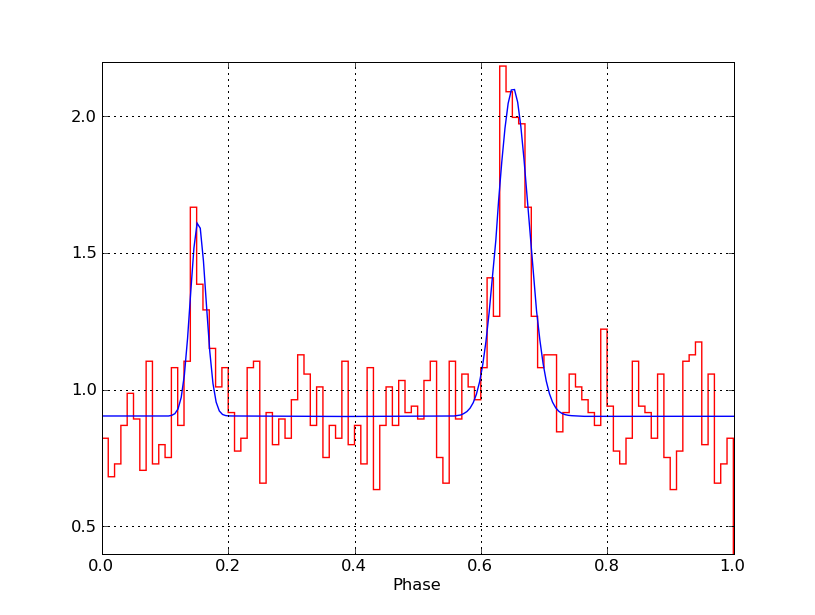
\includegraphics[width=1\textwidth]{plots/template_example_gauss.png}

    \column{0.5\textwidth}
    \center{2 Lorenzians}
    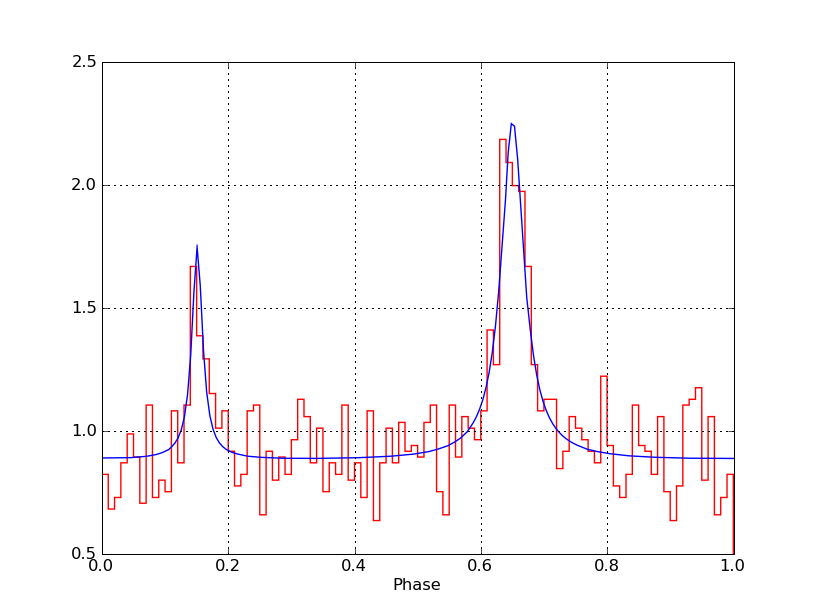
\includegraphics[width=1\textwidth]{plots/template_example_lorentzian.png}
  \end{columns}
\end{frame}

\begin{frame}{Does this work for more complicated pulsars?}
    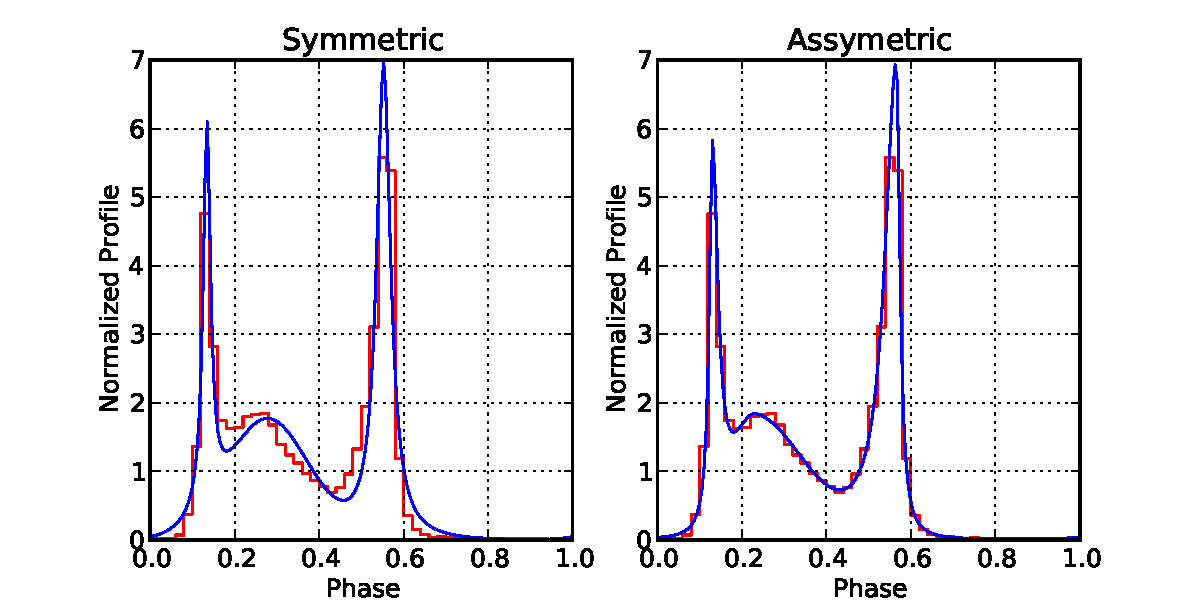
\includegraphics[width=.85\textwidth]{plots/vela.pdf}
  \begin{itemize}
    \item Assymetric 2$\times$Lorenzian + Gaussian $\rightarrow$ surprisingly good fit
      to Vela!
    \item A fairly simple model will hopefully be able to describe all pulsars(?)
    \item This fitting will be done already by PSRCAT2
  \end{itemize}
\end{frame}


\begin{frame}{Hard to define off peak}
  % Plot from /u/gl/lande/work/fermi/pwncatalog/plots_for_bari_f2f/compare_faint_bright

  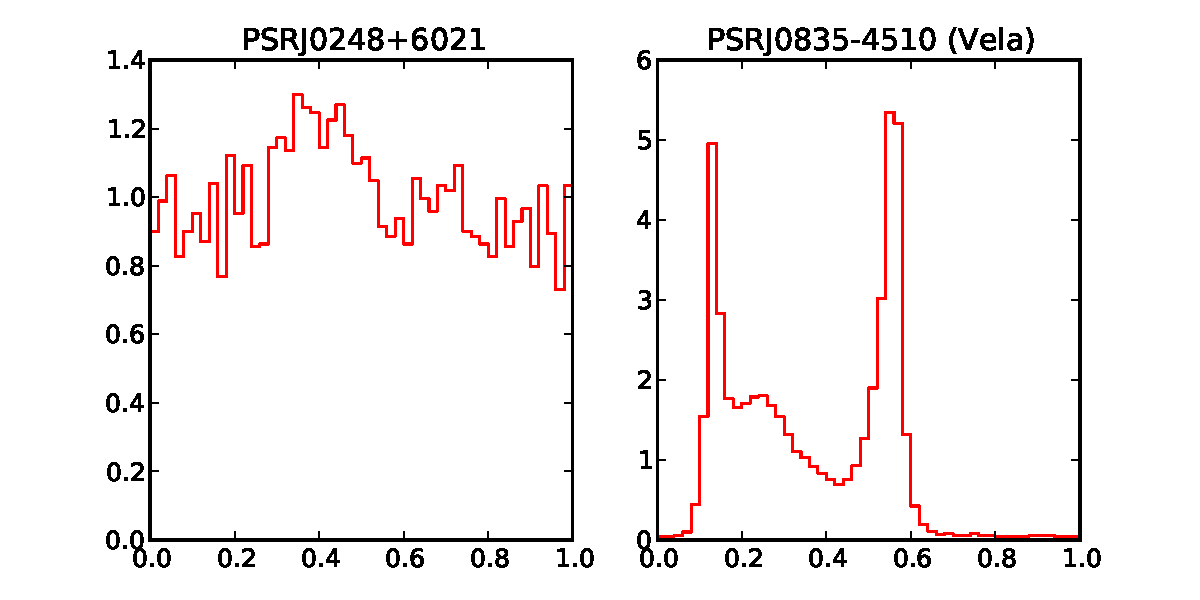
\includegraphics[width=.85\textwidth]{plots/compare_faint_bright.pdf}

  \begin{itemize}
    \item PSRJ0248+6021: TS$_\text{DC}$ = 70 (18M data)
    \item Vela: TS$_\text{DC}$ = 360,000 (18M data) 
    \item Two very different looking phaseograms
    \item How to define the off peak emission?
  \end{itemize}
\end{frame}


\begin{frame}{New method to define off pulse}
\begin{columns}
  \column{0.5\textwidth}
   % taken from http://da.vidr.cc/2008/09/29/creating-flowcharts-with-pgftikz-in-latex/
  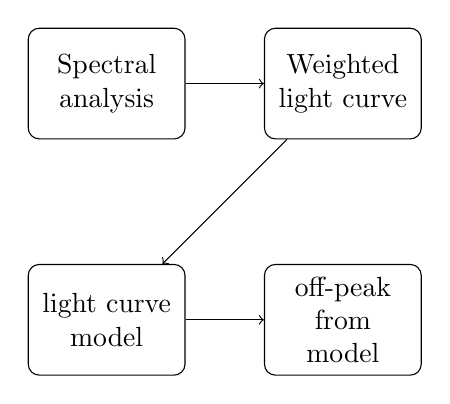
\begin{tikzpicture}[node distance=3cm]
   \node[block] (a)                {Spectral analysis};
   \node[block] (b)  [right of=a]  {Weighted light curve};
   \node[block] (c)  [below of=a]  {light curve model};
   \node[block] (d)  [right of=c]  {off-peak from model};
   \draw[->] (a) -- (b);
   \draw[->] (b) -- (c);
   \draw[->] (c) -- (d);
  \end{tikzpicture}

  \column{0.5\textwidth}


 \begin{itemize}
   \item Everything until ``off-peak from model'' already done by 2nd pulsar catalog (Damien) 
   \item If we could get this to work, it would very nicely sync PSRCAT2 + PWNCAT2 and
     save a lot of duplicate effort
 \end{itemize}
\end{columns}
\end{frame}


\begin{frame}{How does it work?}
  % /u/gl/lande/work/fermi/pwncatalog/plots_for_bari_f2f/find_off_pulse/plot_find_off_pulse.py

\begin{columns}
  \column{0.6\textwidth}
  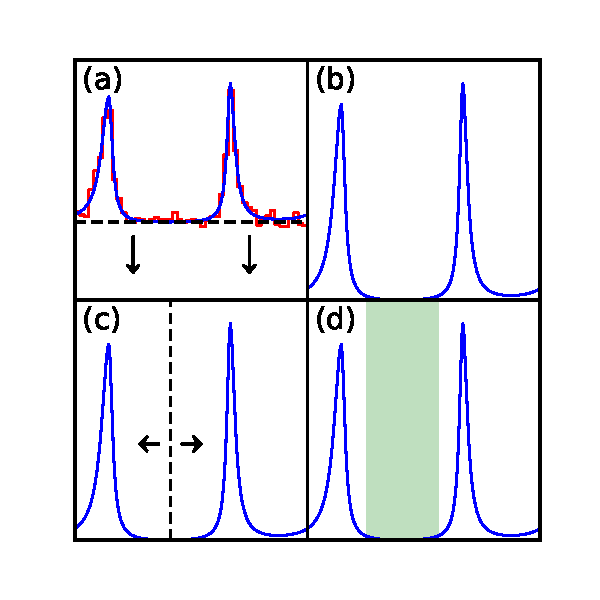
\includegraphics[width=1\textwidth]{plots/find_off_pulse.pdf}
  \column{0.4\textwidth}
  \begin{itemize}
    \item (a) Fit the model
    \item (b) Subtract lowest valley
    \item (c) Guess a center
    \item (d) Integrate until fraction of total emission (say 1\%) is included.
    \item (e) Try many centers $\rightarrow$ pick biggest range
  \end{itemize}
\end{columns}
\end{frame}

\begin{frame}{2 Previous Examples}
  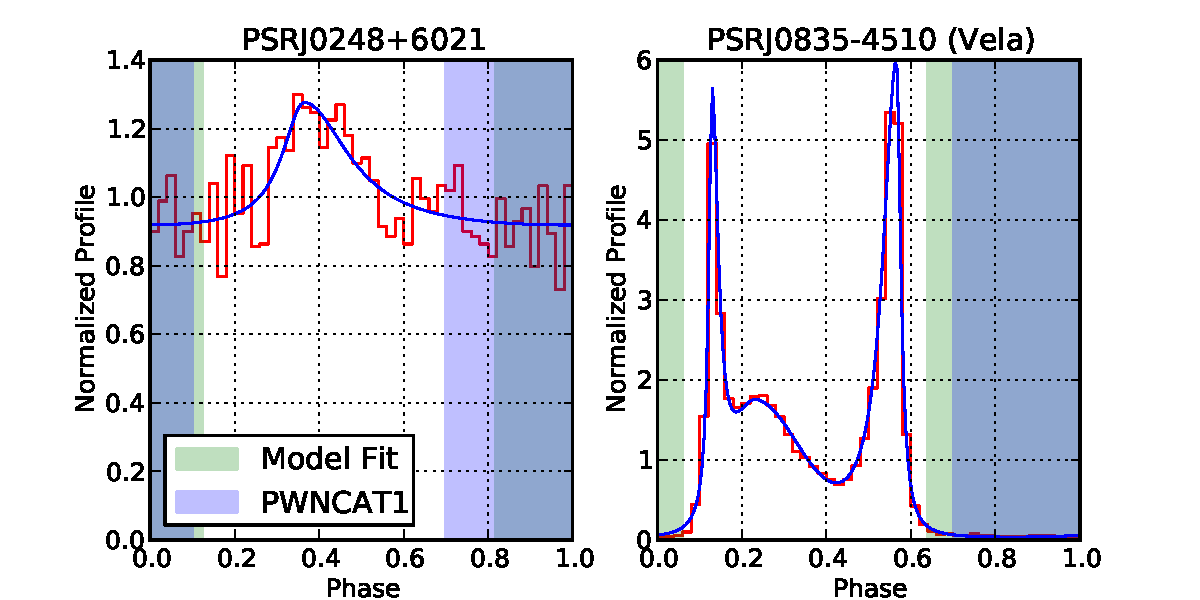
\includegraphics[width=.85\textwidth]{plots/compare_faint_bright2.pdf}

  \begin{itemize}
    \item Integrate out 1\%. 
    \item Qualittivly, works very well
    \item For bright pulsars, 1\% integrates too far (more on this later\dots)
  \end{itemize}
\end{frame}


\begin{frame}{What about Edge cases/Special cases:}

   \begin{columns}
     \column{0.5\textwidth}
  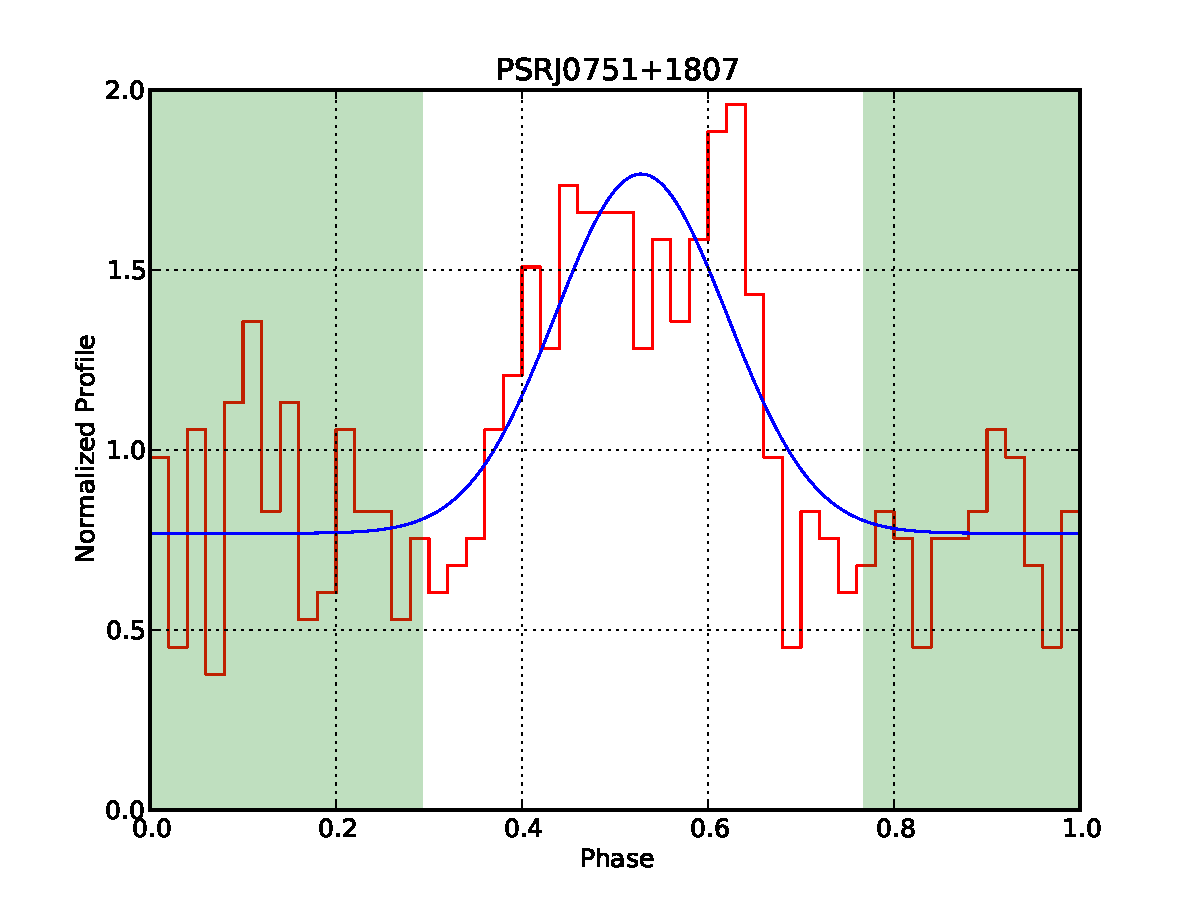
\includegraphics[width=1\textwidth]{plots/edge_case.pdf}
     \column{0.5\textwidth}


  \begin{itemize}
   \item Left Peak is not significant
   \item So would not be included in a pulsar model
   \item But for defining off pulse, should we keep it?
   \item Probably not too important since if the peak is significant, woudl not much bias a PWN analysis
  \end{itemize}
   \end{columns}
\end{frame}


\begin{frame}{Benefits/downsides}
  Benefits:
  \begin{itemize}
    \item Algorithm Fast to run + easy to explain
    \item Algorithm performs what we anyway do by eye anyway
    \item While other algorithms use the off pulse to define
      the on pulse, this method uses the peaks to
      define where there are not peaks
    \item By fitting a physical model, natural way to
      remove statistical flucluations
  \end{itemize}
  Downsides: 
  \begin{itemize}
    \item dependent upon a model of the phaseogram
  \end{itemize}

\end{frame}

\begin{frame}{Determine a second off pulse?}
  \begin{itemize}
    \item For many pulsars (e.g. Vela), bridge emission between two peaks:
    \item For others, could be good second off-peak region to include.
  \end{itemize}
\end{frame}


\begin{frame}{Look at high energy?}
  \begin{itemize}
    \item Is this conservative enough?
    \item Could the peaks be wider at high energy?
    \item Or new peacks at high energy?
    \item As a cross check, should we refit + look for new peaks above 1GeV?
  \end{itemize}
\end{frame}






\begin{frame}{What about very bright pulsars:}

   * 1% of Vela is a lot of source!
   * Should the containment be a function of source brightness?
   * Ideas for containment = 0.01 * (100/TSdc)
      * For vela, TSdc=… so contai
   * Show Vela integrates to 0.01, 0.01 percent, etc.
   * Make a plot of these issues.
   * What about linear decrease: containment.
\end{frame}


\begin{frame}{Conclusion}
  \begin{itemize}
  \item Real test will be how this performs on 108 pulsars + 30 months of data
  \item All code is avalible in \texttt{uw.pulsar.lc\_off\_peak}
  \end{itemize}
\end{frame}

\end{document}
